In this section we will look at a large variety of different simulators, to determine which one best suits our purpose. We will be looking at which operating system and game engine the simulator uses, whether or not it is open source, and the pros and cons of each simulator. 
\\~\\
The purpose of this was to get a good understanding of the different simulators currently in existence. The aim was to find 3-4 simulators that would be worth looking closer at.

%%%%%%%% 4DV-Sim %%%%%%%%%%
\subsection{4DV-Sim}
\textbf{Description:} 4DV-Sim\footnote{Website: https://www.4d-virtualiz.com/en/automotive-simulator/} is a simulator that is designed to emulate the hardware and sensors in autonomous systems. This is a professional product and has a variety of use cases from simulating farming to military.

\textbf{Open Source:} No

\textbf{Operating System:} Linux

\textbf{Game Engine:} Non, but it does use PhysX for the physics engine

\textbf{Pros:} The simulator has a lot of available APIs. The simulator also comes with a configurable GUI to set up the simulation environment how you would like it. Also, as it is professionally made, it looks very good.   

\textbf{Cons:} It is not designed to train machine learning implementations on the simulator, but rather emulate a current hardware setup. Also, as it is not open source, it will not be something that we could modify or expand upon to suit our purposes. 

\textbf{Conclusion:} As 4DV-Sim is not an open-source product it is not something that we can use for this project. It is however interesting to see that simulators like this are needed not just for research purposes, but for customers who want to try out their hardware setup in an emulated environment.


\begin{figure}[H]
    \centering
    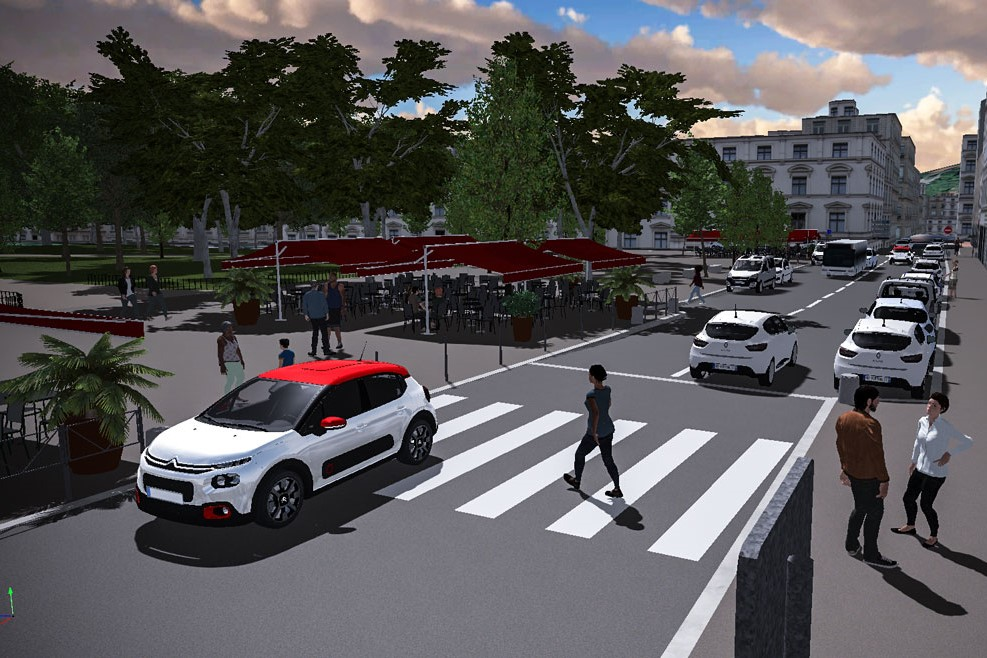
\includegraphics[width=0.5\textwidth]{Simulators/4DV-Sim.jpg}
    \caption{Source: https://www.4d-virtualiz.com/en/automotive-simulator}
\end{figure}

%%%%%%%% AirSIM %%%%%%%%%%
\subsection{AirSim}
\textbf{Description:} AirSim\footnote{Website: https://microsoft.github.io/AirSim/} is a simulator for cars and drones. It is open source and works as a plugin for unreal engine, which means the simulator can be used with any environment which has been modeled inside the game engine. According to their website \cite{AirSim_Website}, the goal of the simulator is to create a platform for AI research to experiment with deep learning, computer vision and reinforcement learning algorithms for autonomous systems. 

\textbf{Open Source:} Yes

\textbf{Operating System:} Any operating system

\textbf{Game Engine:} Primarily Unreal Engine, but it also offers a prototype version in Unity

\textbf{Pros:} Offers a large range of existing APIs. The simulator also has an active community on both discord and Github. It also gives the option to add drones. It is also designed to train machine learning algorithms on it.

\textbf{Cons:} The simulator is not as realistic as other simulators. The vehicle physics is not as good as some of the other simulators, for example the handling and collisions. Also, currently, there are no pedestrians in the game. 

\textbf{Conclusion:} AirSim is worth looking closer into. As it is built using a game engine it should not be too hard to add the missing features, like for example adding and controlling pedestrians. Also, realistic vehicle physics was determined not to be an important factor for this project. 

\begin{figure}[H]
    \centering
    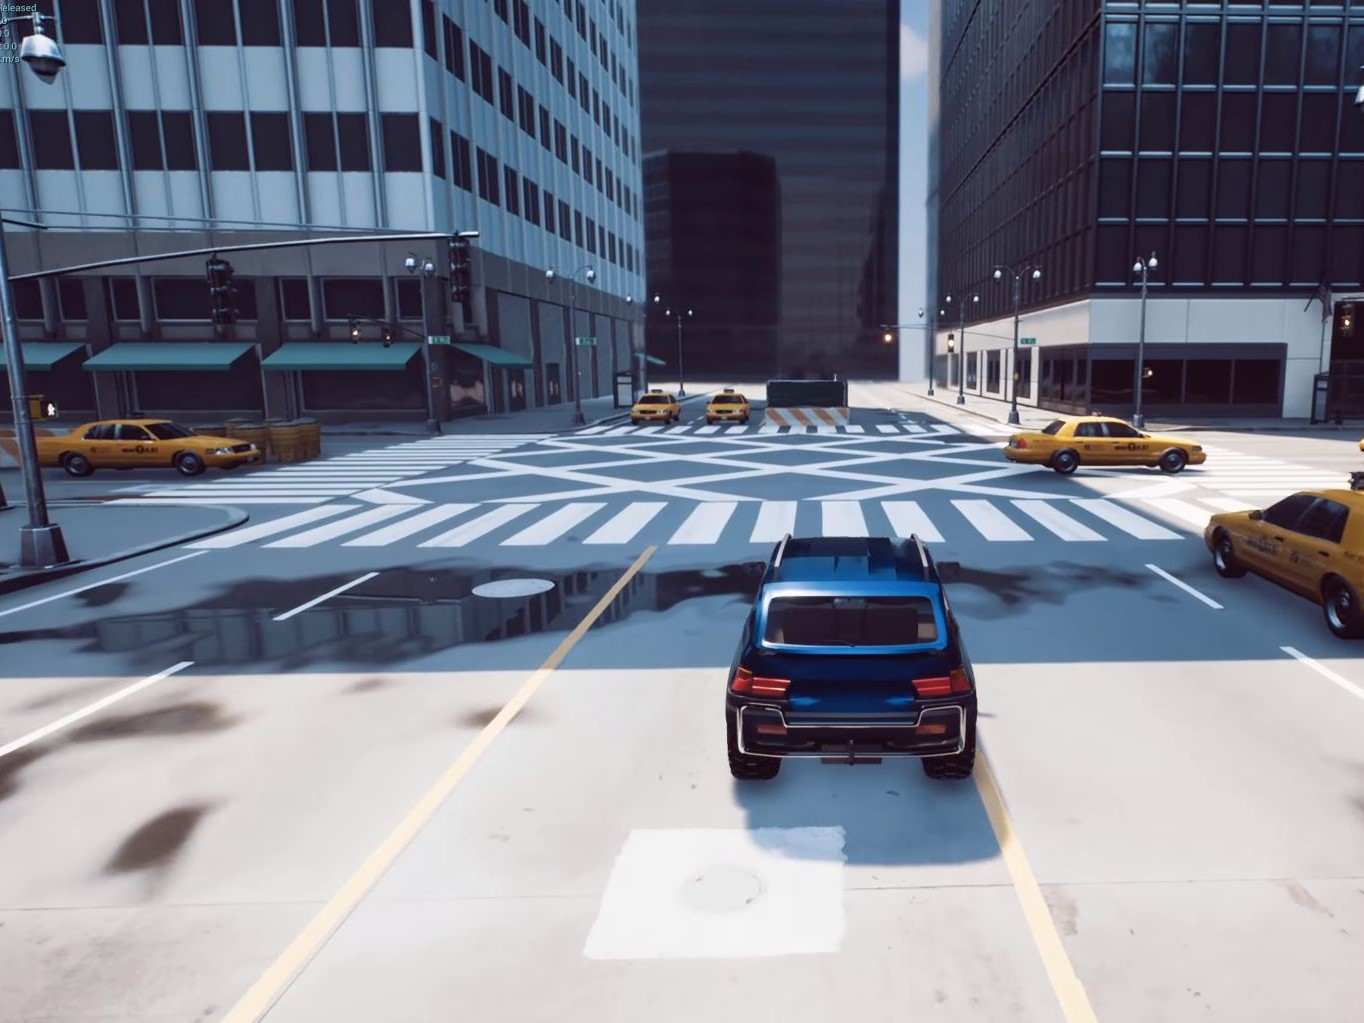
\includegraphics[width=0.5\textwidth]{Simulators/AirSim.JPG}
    \caption{Source: https://microsoft.github.io/AirSim/}
\end{figure}

%%%%%%%% Apollo %%%%%%%%%%
\subsection{Apollo}
\textbf{Description:} Apollo is a simulator which is designed emulate the hardware in autonomous vehicles so that it can be trained for machine learning algorithms. According to their website \cite{Apollo_Website}, Apollo is a flexible architecture which accelerates the development and testing of autonomous vehicles.

\textbf{Open Source:} Yes

\textbf{Operating System:} Any system that can run Docker

\textbf{Game Engine:} Unity

\textbf{Pros:} Accurately models the vehicle physics to help improve the machine leaning algorithms accuracy. The simulator is also actively being worked on by a large community.  

\textbf{Cons:} It looks like quite a complex simulator, and it does therefore not seem like it will be easy to modify. The product is really specific towards training autonomous vehicles. 

\textbf{Conclusion:} Due to the complexity of this simulator, it does not look like something that we could build upon for this project. 

\begin{figure}[H]
    \centering
    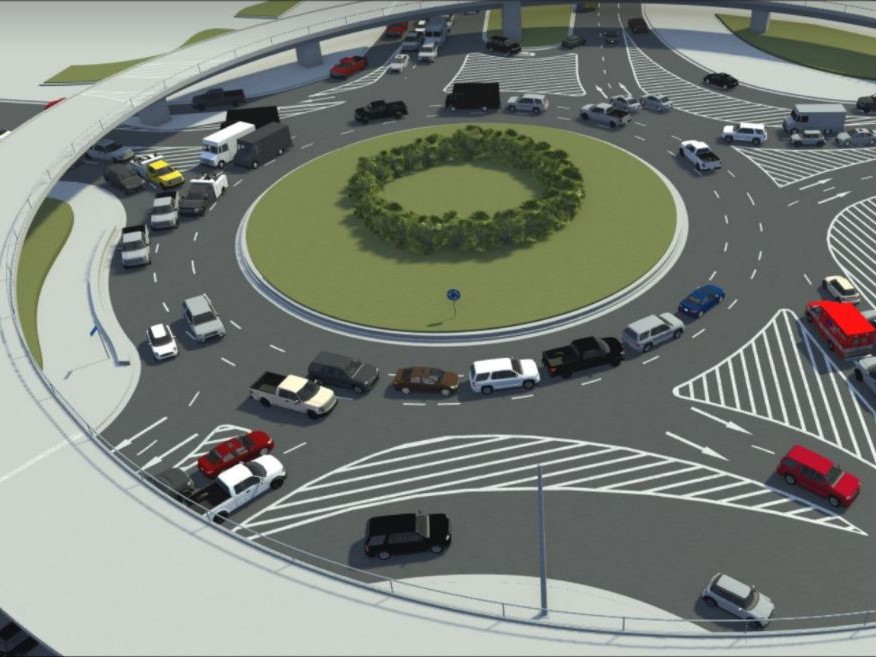
\includegraphics[width=0.5\textwidth]{Simulators/Apollo.JPG}
    \caption{Source: Slide deck from Apollo Game Engine Based Simulation Talk at GDC 2019 - https://bit.ly/2VSzwlF}
\end{figure}

%%%%%%%% Autoware %%%%%%%%%%
\subsection{Autoware}
\textbf{Description:} Autoware is an open-source software for autonomous vehicles. It comes with a large variety of APIs  \cite{Autoware_doc_Website}. Autoware is however not a simulator, but can be used on a simulated vehicle to make it autonomous.

\textbf{Open Source:} Yes

\textbf{Operating System:} Robot Operating System (ROS)

\textbf{Game Engine:} Na

\textbf{Pros:} As it runs on ROS it can easily be adapted to work on a real autonomous vehicle.

\textbf{Cons:} Currently it only works with a specific car model and sensor set up. The software also seems quite complex, and combining it with a simulator will probably be quite challenging.

\textbf{Conclusion:} As this is not a simulator this is not something that we can use for this project. We will see with the LGSVL simulator (\ref{LGSVL_Simulator}), this software can be used along side a simulator to model the autonomous system. 


%%%%%%%% Carla %%%%%%%%%%
\subsection{Carla}
\textbf{Description:} Carla is an open-source simulator for developing autonomous vehicles. It contains a variety of APIs and is actively being developed. Carla is also designed for training machine learning algorithms. 

\textbf{Open Source:} Yes

\textbf{Operating System:} Primarily Ubuntu, but also Windows

\textbf{Game Engine:} Unreal Engine

\textbf{Pros:} Has a lot of features already implemented, such as sensors, vehicle API and the ability to add new objects. Active community. Well documented and lots of information online. 

\textbf{Cons:} Difficult to add new and custom maps. Vehicle handling is not as realistic as some of the other simulators.

\textbf{Conclusion:} Carla is worth looking into further as it has most of the features that we are looking for.


\begin{figure}[H]
    \centering
    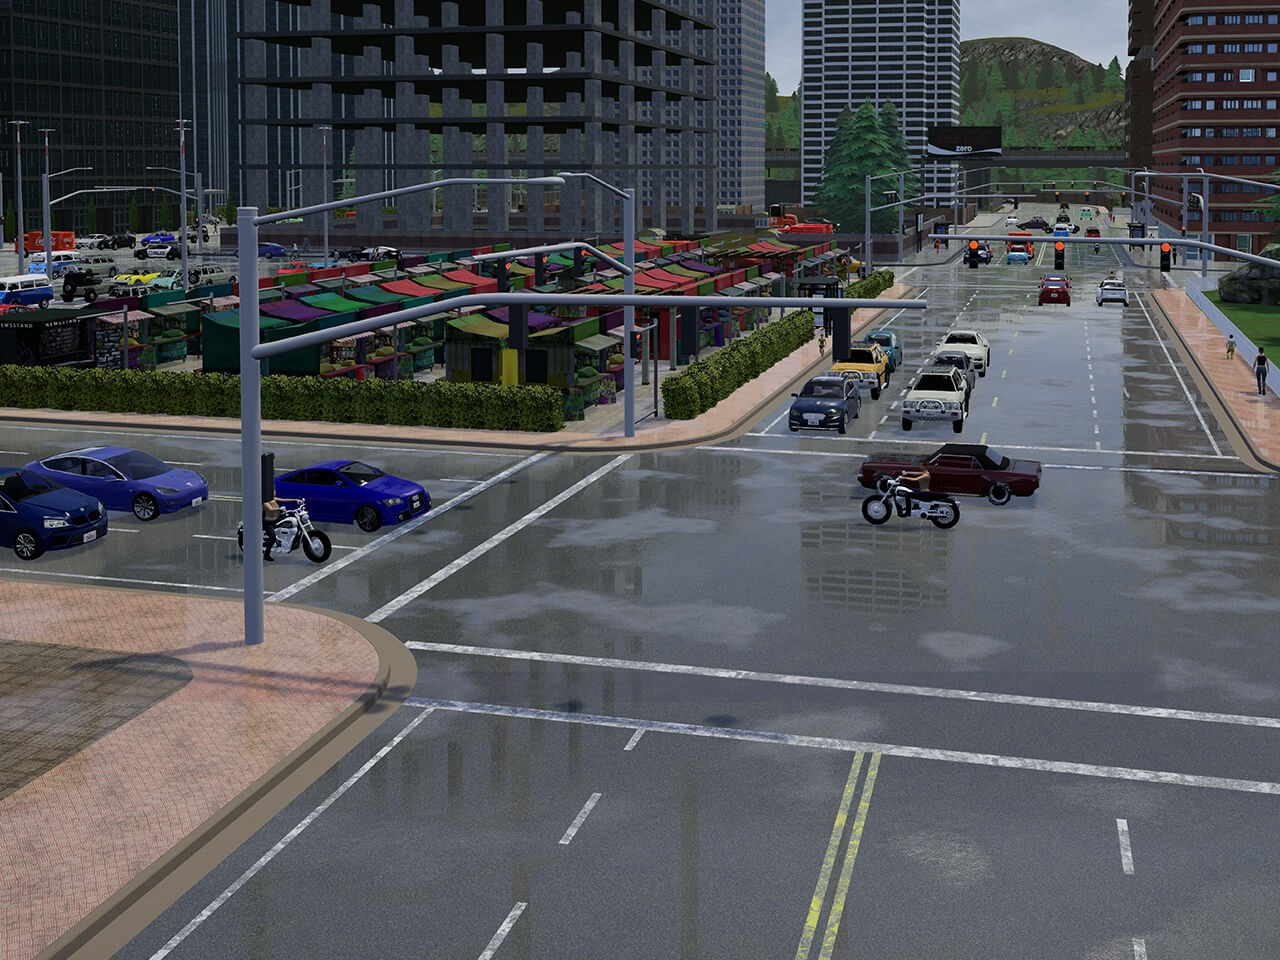
\includegraphics[width=0.5\textwidth]{Simulators/Carla.JPG}
    \caption{Source: https://www.unrealengine.com/en-US/spotlights/carla-democratizes-autonomous-vehicle-r-d-with-free-open-source-simulator}
\end{figure}


%%%%%%%% CrowdSim3D %%%%%%%%%%
\subsection{CrowdSim3D}
\textbf{Description:} CrowdSim3D is primarily a simulator for modeling large crowds, but can also be used for vehicle traffic. 

\textbf{Open Source:} No (£180)

\textbf{Operating System:} Any operating system

\textbf{Game Engine:} Not specified

\textbf{Pros:} Has the ability to control several pedestrians and veichles in a shared space.

\textbf{Cons:} Does not look to be design for machine learning algorithms. Difficult to add new models. Also, as it is not open source it will not be possible to customise the product. 

\textbf{Conclusion:} CrowdSim3D is not worth considering as we cannot adapt the prouct as it is not open source. 

\begin{figure}[H]
    \centering
    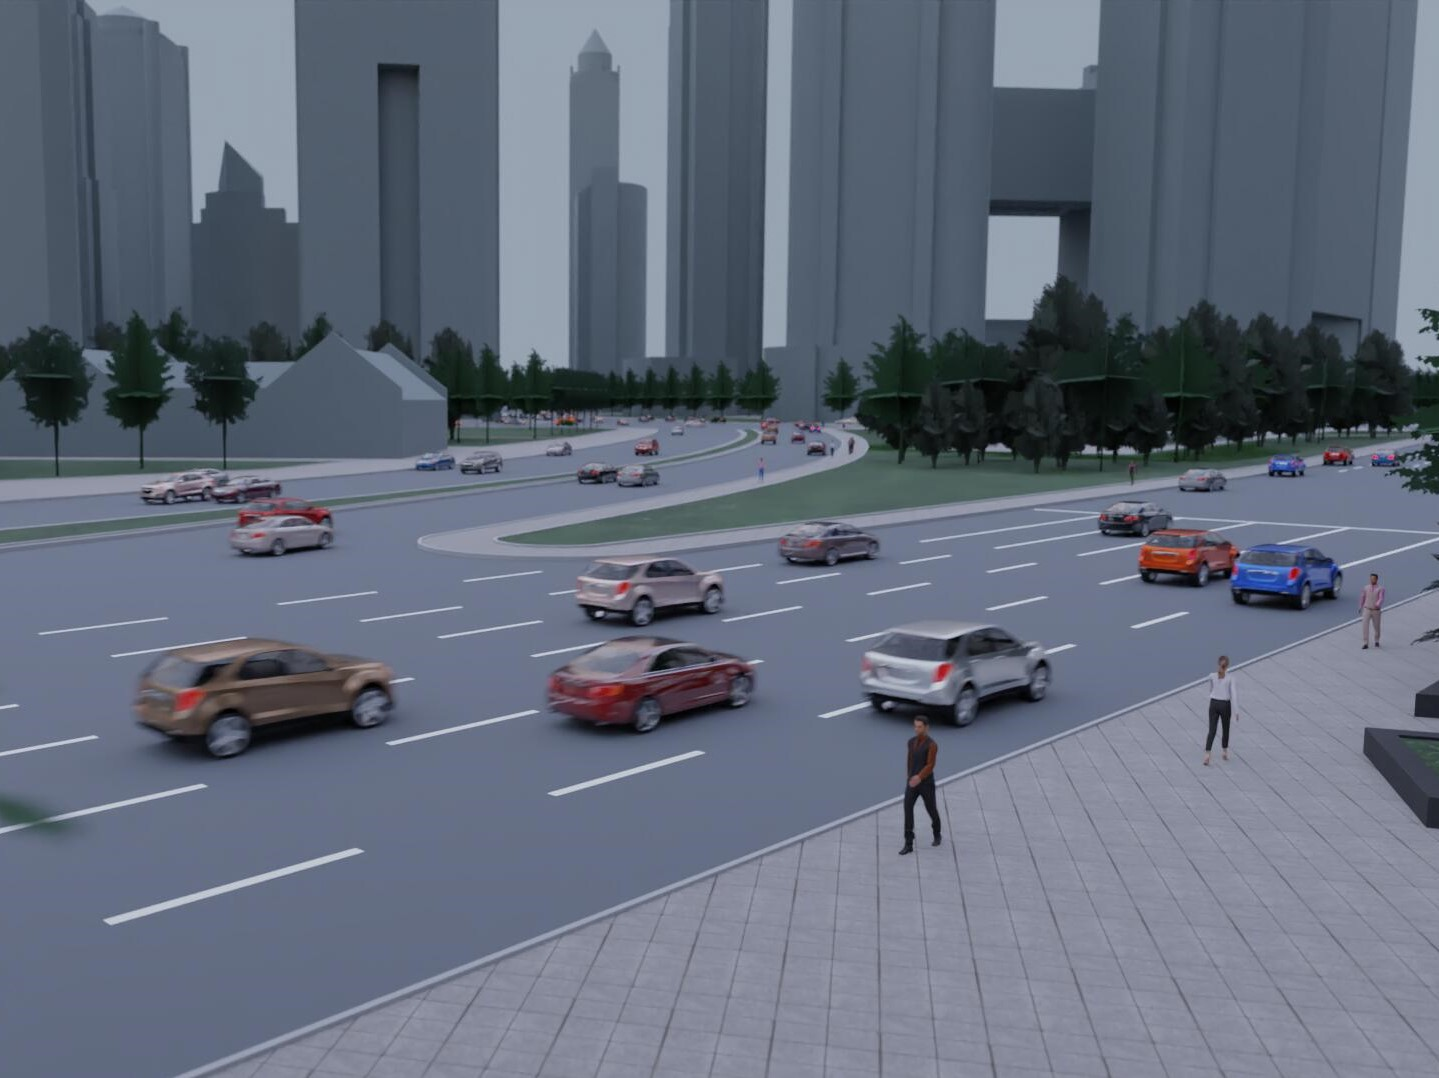
\includegraphics[width=0.5\textwidth]{Simulators/CrowdSim.JPG}
    \caption{Source: https://crowdsim3d.com}
\end{figure}


%%%%%%%% Deep Drive %%%%%%%%%%
\subsection{Deep Drive}
\textbf{Description:} test

\textbf{Open Source:}

\textbf{Operating System:}

\textbf{Game Engine:}

\textbf{Pros:} Is able to handle a variety of different sensors and vehicle setups. 

\textbf{Cons:} Currently there are three maps available, but it is not easy to add your own maps. 

\textbf{Conclusion:} 

\begin{figure}[H]
    \centering
    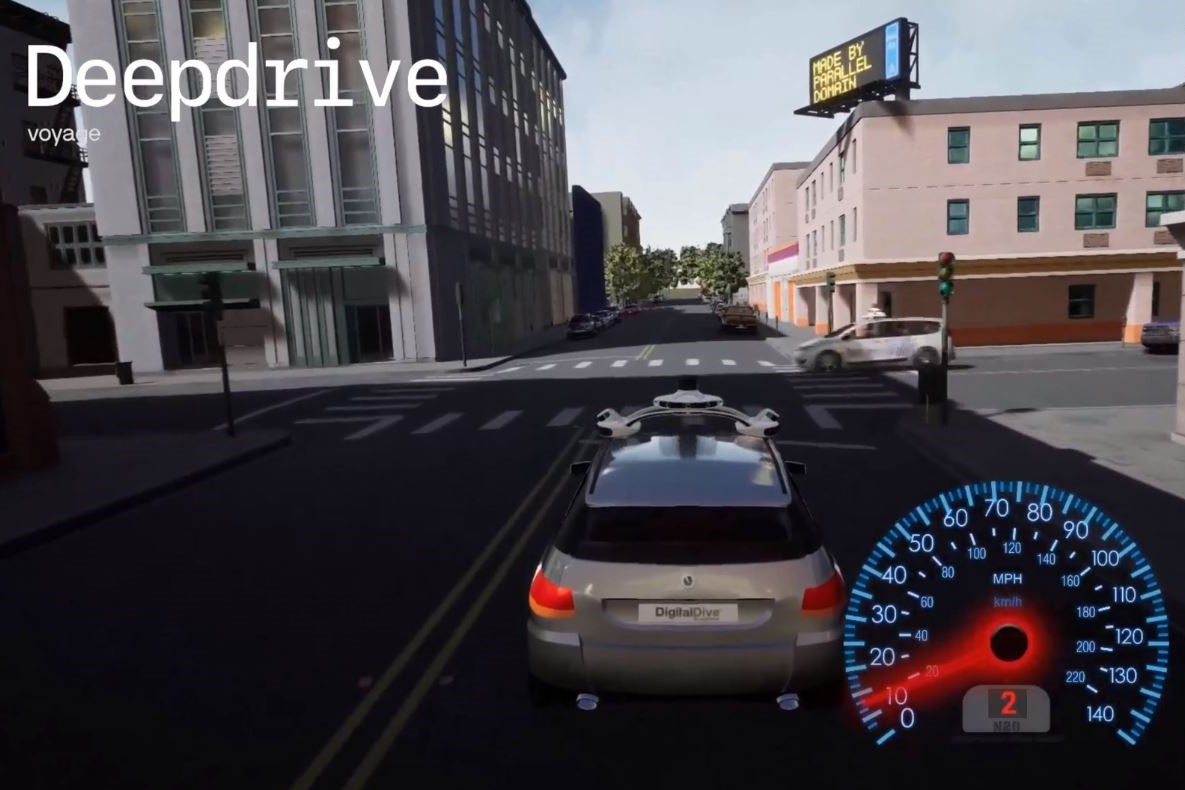
\includegraphics[width=0.5\textwidth]{Simulators/DeepDrive.JPG}
    \caption{Source: https://deepdrive.voyage.auto}
\end{figure}

%%%%%%%% Donkey Car Simulator %%%%%%%%%%
\subsection{Donkey Car Simulator}
\textbf{Description:} test

\textbf{Open Source:}

\textbf{Operating System:}

\textbf{Game Engine:}

\textbf{Pros:}

\textbf{Cons:}


%%%%%%%% Gazebo %%%%%%%%%%
\subsection{Gazebo}
\textbf{Description:} test

\textbf{Open Source:}

\textbf{Operating System:}

\textbf{Game Engine:}

\textbf{Pros:}

\textbf{Cons:}


%%%%%%%% LPZRobots %%%%%%%%%%
\subsection{LPZRobots}
\textbf{Description:} test

\textbf{Open Source:}

\textbf{Operating System:}

\textbf{Game Engine:}

\textbf{Pros:}

\textbf{Cons:}


%%%%%%%% LGSVL Simulator %%%%%%%%%%
\subsection{LGSVL Simulator} \label{LGSVL_Simulator}
\textbf{Description:} test
% Uses Apollo and Autoware

\textbf{Open Source:}

\textbf{Operating System:}

\textbf{Game Engine:}

\textbf{Pros:}

\textbf{Cons:}

%https://github.com/lgsvl/simulator

%%%%%%%% Marliou %%%%%%%%%%
\subsection{Marliou}
\textbf{Description:} test

\textbf{Open Source:}

\textbf{Operating System:}

\textbf{Game Engine:}

\textbf{Pros:}

\textbf{Cons:}

%%%%%%%% MRDS - Microsoft Robotics Developer Studio %%%%%%%%%%
\subsection{MRDS - Microsoft Robotics Developer Studio}
\textbf{Description:} test

\textbf{Open Source:}

\textbf{Operating System:}

\textbf{Game Engine:}

\textbf{Pros:}

\textbf{Cons:}


%%%%%%%% rFpro %%%%%%%%%%
\subsection{rFpro}
\textbf{Description:} test

\textbf{Open Source:}

\textbf{Operating System:}

\textbf{Game Engine:}

\textbf{Pros:}

\textbf{Cons:}

%%%%%%%% Rigs of Rods %%%%%%%%%%
\subsection{Rigs of Rods}
\textbf{Description:} test

\textbf{Open Source:}

\textbf{Operating System:}

\textbf{Game Engine:}

\textbf{Pros:}

\textbf{Cons:}

%%%%%%%% TORCS - The Open Racing Car Simulator %%%%%%%%%%
\subsection{TORCS - The Open Racing Car Simulator}
\textbf{Description:} test

\textbf{Open Source:}

\textbf{Operating System:}

\textbf{Game Engine:}

\textbf{Pros:}

\textbf{Cons:}

%%%%%%%% Webots %%%%%%%%%%
\subsection{Webots}
\textbf{Description:} test

\textbf{Open Source:}

\textbf{Operating System:}

\textbf{Game Engine:}

\textbf{Pros:}

\textbf{Cons:}


\subsection{Conclusion?}